\section{Introduction}
\label{sec:intro}
\begin{comment}
1. graphs are big and getting bigger. the workloads are varied
2. Databases storing the full dataset (graph or unmined Relational) are ground truth
2. The workloads are serviced by different classes of systems -- separate evolution of GPS and GDB. GDB is the ground truth and GPS needs ETL/PP
3. Each system is specialized for it's own workload and underperforms on the other set. This is a problem. 
4. 
\end{comment}
\textbf{Large graphs are now ubiquitous, and more than a decade of research has investigated how to store and process them efficiently.}
Graphs are a natural and common data model to represent relationships between entities in various applications, including social networks, the World Wide Web, recommendation systems, fraud detection, and biological networks~\cite{ubiquityLargeGraphsVLDB2017}.
It is increasingly common to store and analyze graphs with billions of nodes and trillions of edges, and there has been significant research and commercial effort devoted to designing systems to store and process large graphs~\cite{ching2015oneTrillion,besta2020demystifying, lin2018shentu, gupta2024graphscale, zhou2025redtao}.
The nodes and edges of a graph may be of different types (i.e., they have labels), and each might be further annotated with collections of attributes (i.e., properties)~\cite{besta2020demystifying}.
The nodes and edges together form the \emph{structure} of the graph, while the labels and properties give the graph \emph{semantic meaning}.

\textbf{Graph workloads fall into categories similar to those used to classify conventional database workloads}.
OLTP queries on graphs are similar to OLTP queries on tabular data; for example, in a social network, a user might wish to see the latest posts and replies on their favorite ongoing Twitter feud~\cite{AholeMusk:online}.
Such \emph{interactive} queries are latency sensitive, and many real-time analytics applications, such as fraud detection in financial networks, demand low latency, typically bounded at about 20 ms~\cite{qiu2018real}.
Analytical workloads on graphs (Graph OLAP) are queries that can be answered only through ``whole-graph'' analysis.
Graph OLAP tasks analyze the graph structure and are therefore run on a ``structural graph'' and typically ignore the associated labels and properties.
% that is generated by selecting the relevant nodes and edges (filtering on labels) and ignoring any unimportant properties; we call these materialized graphs structural graphs.
For example, Twitter's recommendation teams run PageRank and topic similarity tasks on the user-follow graph to suggest new users to follow~\cite{tang2022taming}.
These tasks must interact with large parts of the graph, if not the whole graph, and will typically take longer to finish than graph OLTP queries.
These two different types of workloads are typically run on different classes of systems: graph databases for graph OLTP workloads and specialized graph processing systems for graph OLAP.
This dual-silo approach entails substantial ETL overhead and consistency challenges, presenting a compelling case for a more integrated graph processing paradigm.

% \textbf{Databases are the primary data store for graphs.}
% Extensive research and several products have shown that it is feasible to use relational databases to store graphs~\cite{bronson2013tao,hong2015pgx,OraclePG,WhatIsOracleSpatialGraph:online,graphProcessingRDBMS,duckpgq:online,welc2013graph, hong2013early}.
% If we store the graph only in its relational form, relations (edges) are encoded as joins, and graph traversals become recursive self-joins~\cite{10.1145/3129246}.
% As a result, RDBMSs do not perform well for graph analysis tasks, as the computation of these recursive self-joins is expensive~\cite{TransitiveClosureBiskupStiefeling1989}.
% Specialized RDBMS' with graph libraries such as PGX\cite{hong2015pgx,hong2013early} perform well on graph analytics, but essentially perform the 
% In response to this mismatch between graph analysis tasks and relational databases, we have witnessed an explosion in special-purpose systems for storing and processing graph-structured data.

\textbf{Databases are the primary data store for graphs.} 
Large-scale graphs typically originate in, and are managed by, relational or key-value databases, and substantial effort has gone into enabling graph analytics from within these systems.
One line of work stores graphs in relational tables and routes analytics to a separate in-memory engine: Facebook's TAO~\cite{bronson2013tao} serves the social graph from MySQL but delegates analytics to offline pipelines; Oracle stores property graphs in relational tables and loads them into PGX, an in-memory graph server, for analysis~\cite{OraclePG,WhatIsOracleSpatialGraph:online,hong2015pgx,welc2013graph,graphProcessingRDBMS,hong2013early}.
A complementary line extends SQL with graph syntax, most notably SQL/PGQ~\cite{duckpgq:online}. 
In these systems, pattern matching and path queries can be expressed over relational tables, but these extensions build only transient in-memory representations and offer no persistent graph layout or transactional mutation support.
When the graph remains in purely relational form, traversals reduce to recursive self-joins whose cost grows with path length~\cite{10.1145/3129246,TransitiveClosureBiskupStiefeling1989}, and in every case analytics still requires either a dedicated in-memory engine or an ad-hoc in-memory construction step.
None of these approaches provides a single persistent store with analytics-friendly graph layouts and integrated transactional mutation support.
In response to this mismatch between graph analysis tasks and relational databases, we have witnessed an explosion in special-purpose systems for storing and processing graph-structured data.

Specialized graph databases such as Neo4j~\cite{neo4j} and ArangoDB~\cite{arangodb} follow the tradition of relational databases, providing a schema-oriented organization and a high-level query language.
These systems work well for OLTP workloads, but frequently exhibit suboptimal performance on OLAP tasks.
In contrast, a second class of graph processing systems, such as Pregel~\cite{malewicz2010pregel}, GraphX~\cite{gonzalez2014graphx}, PowerLyra~\cite{powerlyra2019}, GraphChi~\cite{kyrola2012graphchi} and Ligra~\cite{shun2013ligra}, are specifically designed to provide outstanding OLAP performance, but typically do not provide OLTP-style query capabilities.
% These graph processing systems accept a structural graph, which must then be preprocessed to construct a performant in-memory or on-disk layout.
Preparing the data for processing with one of these special-purpose systems requires that we extract the structural graph from the database, transform it into a form amenable to ingestion, and then load the data into the graph processing system.
\textit{This is the central dichotomy of graph processing systems}: graph databases allow for \emph{persistent storage} of graphs in a native representation but are outperformed on OLAP workloads by specialized graph processing systems, which need a costly ingest and preprocessing phase before executing efficient graph analytics queries.

% \textbf{Neither graph databases nor graph processing systems handle all graph workloads efficiently.}
% While graph databases offer the data management capabilities that are needed to efficiently organize and query graphs, they underperform on whole graph analytics tasks\PM{insert citations. maybe even a plot?}.
% Purpose-built custom graph processing systems are orders of magnitude faster, but they need to be provided data from the primary data source (graph or relational database) which then needs to be preprocessed into a layout (in-memory or on-disk) that is amenable to analytics.
% This extract-transform-load (ETL) and pre-processing heavy initial step in graph analytics quickly becomes a bottleneck and often takes longer to complete than the actual analytics task itself~\PM{citation/table}.
% Each new batch of updates or graph snapshot requires reconstruction of the graph layout, which only makes the pre-analytics overhead worse. 
% \textit{This is the central dichotomy of graph processing systems}: graph databases allow for persistent storage of graphs in a native representation, but they are outperformed by specialized graph processing systems, which need a costly ingest and preprocessing phase before executing efficient graph analytics queries.

% \textbf{There is a clear need to build Hybrid Graph Transactional and Analytical Processing (HGTAP) systems.}
\textbf{This dichotomy led to the development of Hybrid Graph Transactional and Analytical Processing (HGTAP) systems, such as LiveGraph~\cite{zhu2019livegraph} and GART~\cite{shen2023bridging}.}
LiveGraph uses a custom data layout based on adjacency lists stored in a large memory-mapped region (considered harmful~\cite{crotty2022you}).
However, despite using analytics-friendly data layout, LiveGraph has a low transaction throughput and poor OLAP performance because their transaction manager fails to scale well~\cite{libinzhou2025GTX}.
On the other hand, GART constructs an in-memory multi-versioned CSR that is limited by the memory capacity.
% We show that a persistent graph database can deliver the OLTP performance expected from a database together with the OLAP performance expected from a purpose-built graph processing system.

We studied the graph data management landscape and observed the following:
1$)$ The vast majority of the time in graph analytics is spent creating the in-memory or on-disk data layouts. 
2$)$ Managing the dynamism in graph data requires the use of a transaction manager, which comes with a great engineering overhead.
3$)$ Neither in-memory systems nor out-of-core systems can efficiently handle the large graphs that are commonplace. Distributed graph processing is an option, yet suffers from severe communication overhead~\cite{mcsherry2015scalability,beamer2016understanding} and poor work balance~\cite{hajidehi2023cuttana}.
% 4$)$ One data layout does not fit all workloads, and there is a need to create analytics-friendly persistent layouts that do not lead to reduced graph OLTP performance. 
4$)$ Data layout is the key determinant of system performance. An analytics-friendly persistent layout can be extended to store full property graphs; we demonstrate this with a typed property storage layer that achieves property-mutation latencies three to four orders of magnitude lower than established graph databases.
5$)$ Each system is designed for a specific operating condition (in-memory or out-of-core, static or dynamic graphs), but none transcend the full spectrum of use-cases.\PM{somebody help me reframe this.}

\textbf{\project{} is a hybrid transactional and analytical graph database that matches the performance of in-memory graph processing systems without data movement or preprocessing, while also delivering high insertion throughput and efficient, columnar property graph storage.}
It is a single-node system built on the \wt{}~\cite{WiredTigerDocumentation} key/value store, which provides \project{} with a mature transaction manager, write-ahead log, and buffer pool at no additional engineering cost.
\project{} provides two structural layouts that produce sequential iterator-based read performance for analytics, and extends them with a typed property storage layer supporting both embedded and columnar storage modes.
Insertion throughput scales near-linearly to 72 threads, sustaining up to 1.48\,M edges/sec on the write-optimized layout ($3\times$ higher than LiveGraph~\cite{zhu2019livegraph}), while property-mutation latencies are three to four orders of magnitude lower than established graph databases such as Neo4j~\cite{neo4j} and JanusGraph\cite{janusgraph}.
\preliminary{Preliminary results on concurrent insertion and analytics show that analytics latency remains competitive at moderate write ratios, with \project{} sustaining $1.8\times$ the mixed-workload write throughput of LiveGraph at the balanced operating point.}
We modified GAPBS~\cite{beamer2015gap} to use our API and show that our end-to-end analytics performance is competitive with in-memory systems, while scaling to out-of-core graphs.
\project{} is uniquely flexible across the whole spectrum of operating conditions \PM{this needs better phrasing} and delivers robust $($if not the best$)$ performance uniformly.

\begin{figure}[t]
  \centering
  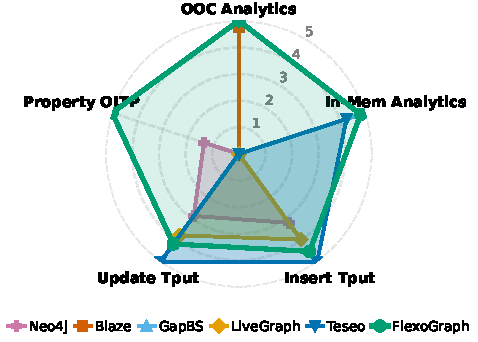
\includegraphics[scale=0.60]{content/fig/spider_chart.pdf}
  \caption{Flexograph delivers robust performance across the entire spectrum of operating conditions common in graph data management.}
  \label{fig:fg-spider}
\end{figure}

\textbf{Our contributions} are as follows.
\begin{itemize}
  \item We present a hybrid graph database that delivers robust performance on whole-graph analytics, transactional queries, and property graph operations without ETL or preprocessing.
  \item A principled analysis of analytics-friendly data layouts and how a mature key-value store (\wt{}~\cite{WiredTigerDocumentation}) can serve as the storage engine for a graph database.
  \item A typed property storage layer with embedded and columnar modes that achieves property-mutation latencies three to four orders of magnitude lower than that of Neo4j, JanusGraph, and ArangoDB.
  \item The design of efficient, read-only neighborhood iterators on graph snapshots for implementing analytics algorithms, and a flexible partitioning strategy that splits work between threads by vertex count or edge count.
  \item Insertion throughput that scales near-linearly to 72 threads, sustaining up to 1.48\,M edges/sec ($3\times$ LiveGraph). Preliminary mixed-workload results show that analytics latency remains competitive under concurrent insertion at moderate writer ratios.
  \item We show that \project{} matches the analytics performance of in-memory and out-of-core graph processing systems while also achieving the transactional performance of in-memory dynamic graph containers.
\end{itemize}


% As the amount of graph structured data continues to grow, the capital expenditure required for processing these datasets is also increasing correspondingly.
% For example, Google reports using a cluster with 128TB of aggregate RAM and ~1000 compute nodes to compute connected components on a graph with a billion nodes and trillion edges~\cite{stergiou2018shortcutting}.
% Similarly, Alibaba's GraphScope reports using an 8 node cluster with two 26 core Xeon Platinum CPUs and 768GBs of aggregate RAM to run graph analytics on Graphs with at most a billion edges~\cite{fan2021graphscope}.
% Several distributed in-memory graph processing systems surprisingly underperform compared to single-threaded implementations due to high communication cost~\cite{mcsherry2015scalability,beamer2016understanding} and poor work balance~\cite{hajidehi2023cuttana}.
% These drawbacks of multi-machine and in-memory systems prompted the development of out-of-core systems that can process larger-than-memory datasets by efficiently using secondary storage ~\cite{kyrola2012graphchi,roy2013x, reducedDiskIO2017Ai,maass2017mosaic,zhu2015gridgraph,zhang2018wonderland,zheng2015flashgraph,kim2022blaze,ai2018clip}.
% These systems have been designed for machines that have a limited memory budget but several CPU cores, and focus on maximizing the disk bandwidth utilization.
% Out-of-Core systems can outperform multi-machine systems, but are still slower than state-of-the-art in-memory systems.
